% generated by Plantuml 1.2024.2       
\definecolor{plantucolor0000}{RGB}{0,0,0}
\definecolor{plantucolor0001}{RGB}{241,241,241}
\definecolor{plantucolor0002}{RGB}{24,24,24}
\definecolor{plantucolor0003}{RGB}{180,167,229}
\definecolor{plantucolor0004}{RGB}{173,209,178}
\definecolor{plantucolor0005}{RGB}{200,41,48}
\definecolor{plantucolor0006}{RGB}{132,190,132}
\definecolor{plantucolor0007}{RGB}{3,128,72}
\definecolor{plantucolor0008}{RGB}{254,255,221}
\definecolor{plantucolor0009}{RGB}{235,147,127}
\scalebox{0.6}{
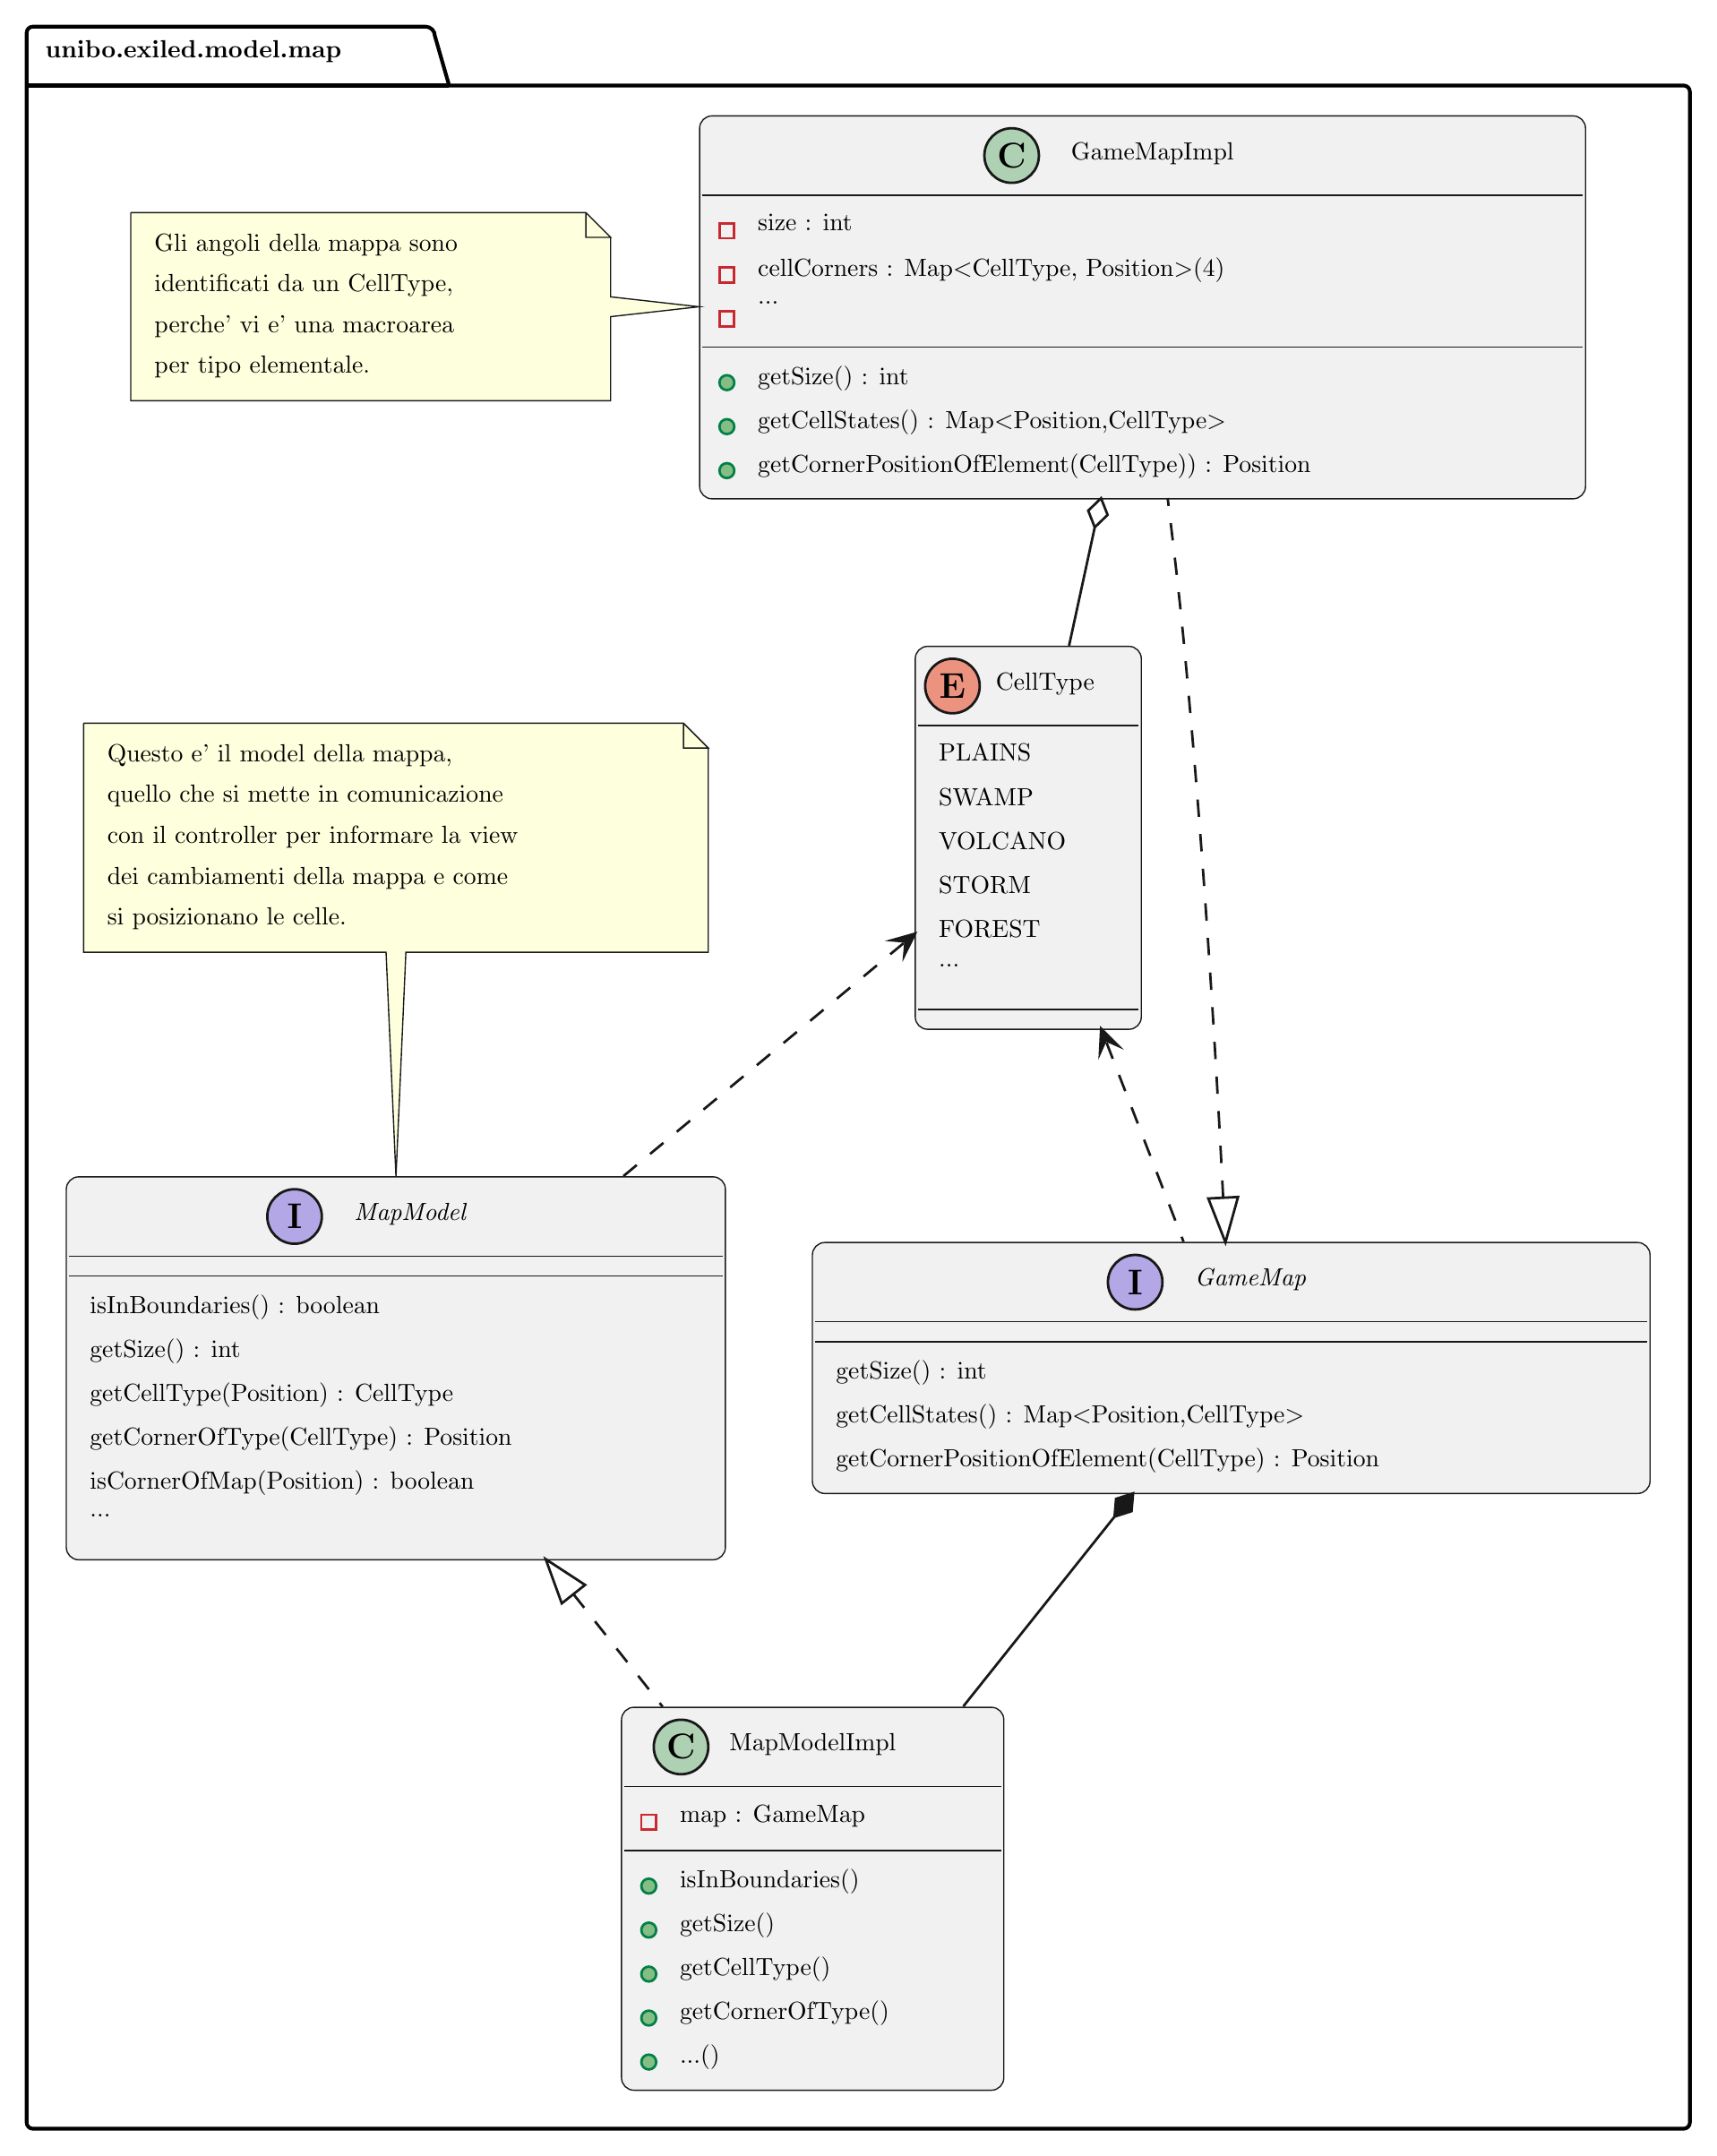
\begin{tikzpicture}[yscale=-1
,pstyle0/.style={color=black,line width=1.5pt}
,pstyle1/.style={color=plantucolor0002,fill=plantucolor0001,line width=0.5pt}
,pstyle2/.style={color=plantucolor0002,fill=plantucolor0003,line width=1.0pt}
,pstyle3/.style={color=plantucolor0002,line width=0.5pt}
,pstyle4/.style={color=plantucolor0002,fill=plantucolor0004,line width=1.0pt}
,pstyle5/.style={color=plantucolor0005,line width=1.0pt}
,pstyle6/.style={color=plantucolor0007,fill=plantucolor0006,line width=1.0pt}
,pstyle7/.style={color=plantucolor0002,fill=plantucolor0008,line width=0.5pt}
,pstyle9/.style={color=plantucolor0002,line width=1.0pt,dash pattern=on 7.0pt off 7.0pt}
,pstyle10/.style={color=plantucolor0002,line width=1.0pt}
,pstyle11/.style={color=plantucolor0002,fill=plantucolor0002,line width=1.0pt}
]
\draw[pstyle0] (8.5pt,6pt) -- (166.9483pt,6pt) arc(270:360:3.75pt)  -- (176.4483pt,29.7461pt) -- (674.5pt,29.7461pt) arc(270:360:2.5pt)  -- (677pt,851.5pt) arc(0:90:2.5pt)  -- (8.5pt,854pt) arc(90:180:2.5pt)  -- (6pt,8.5pt) arc(180:270:2.5pt) ;
\draw[pstyle0] (6pt,29.7461pt) -- (176.4483pt,29.7461pt);
\node at (10pt,8pt)[below right,color=black]{\textbf{unibo.exiled.model.map}};
\draw[pstyle1] (323pt,501.5pt) arc (180:270:5pt) -- (328pt,496.5pt) -- (655.9307pt,496.5pt) arc (270:360:5pt) -- (660.9307pt,501.5pt) -- (660.9307pt,592.7383pt) arc (0:90:5pt) -- (655.9307pt,597.7383pt) -- (328pt,597.7383pt) arc (90:180:5pt) -- (323pt,592.7383pt) -- cycle;
\draw[pstyle2] (453.2306pt,512.5pt) ellipse (11pt and 11pt);
\node at (453.2306pt,512.5pt)[]{\textbf{\Large I}};
\node at (473.7306pt,503.627pt)[below right,color=black]{\textit{GameMap}};
\draw[pstyle3] (324pt,528.5pt) -- (659.9307pt,528.5pt);
\draw[pstyle3] (324pt,536.5pt) -- (659.9307pt,536.5pt);
\node at (329pt,540.5pt)[below right,color=black]{getSize() : int};
\node at (329pt,558.2461pt)[below right,color=black]{getCellStates() : Map\textless Position,CellType\textgreater };
\node at (329pt,575.9922pt)[below right,color=black]{getCornerPositionOfElement(CellType) : Position};
\draw[pstyle1] (277.5pt,47pt) arc (180:270:5pt) -- (282.5pt,42pt) -- (629.9071pt,42pt) arc (270:360:5pt) -- (634.9071pt,47pt) -- (634.9071pt,191.4766pt) arc (0:90:5pt) -- (629.9071pt,196.4766pt) -- (282.5pt,196.4766pt) arc (90:180:5pt) -- (277.5pt,191.4766pt) -- cycle;
\draw[pstyle4] (403.3869pt,58pt) ellipse (11pt and 11pt);
\node at (403.3869pt,58pt)[]{\textbf{\Large C}};
\node at (423.8869pt,49.127pt)[below right,color=black]{GameMapImpl};
\draw[pstyle3] (278.5pt,74pt) -- (633.9071pt,74pt);
\draw[pstyle5] (285.5pt,85.373pt) rectangle (291.5pt,91.373pt);
\node at (297.5pt,78pt)[below right,color=black]{size : int};
\draw[pstyle5] (285.5pt,103.1191pt) rectangle (291.5pt,109.1191pt);
\node at (297.5pt,95.7461pt)[below right,color=black]{cellCorners : Map\textless CellType, Position\textgreater (4)};
\draw[pstyle5] (285.5pt,120.8652pt) rectangle (291.5pt,126.8652pt);
\node at (297.5pt,113.4922pt)[below right,color=black]{...};
\draw[pstyle3] (278.5pt,135.2383pt) -- (633.9071pt,135.2383pt);
\draw[pstyle6] (288.5pt,149.6113pt) ellipse (3pt and 3pt);
\node at (297.5pt,139.2383pt)[below right,color=black]{getSize() : int};
\draw[pstyle6] (288.5pt,167.3574pt) ellipse (3pt and 3pt);
\node at (297.5pt,156.9844pt)[below right,color=black]{getCellStates() : Map\textless Position,CellType\textgreater };
\draw[pstyle6] (288.5pt,185.1035pt) ellipse (3pt and 3pt);
\node at (297.5pt,174.7305pt)[below right,color=black]{getCornerPositionOfElement(CellType)) : Position};
\draw[pstyle7] (48pt,81pt) -- (48pt,156.9141pt) -- (48pt,156.9141pt) -- (241.5987pt,156.9141pt) -- (241.5987pt,156.9141pt) -- (241.5987pt,123pt) -- (277.27pt,119pt) -- (241.5987pt,115pt) -- (241.5987pt,91pt) -- (231.5987pt,81pt) -- (48pt,81pt) -- (48pt,81pt);
\draw[pstyle7] (231.5987pt,81pt) -- (231.5987pt,91pt) -- (241.5987pt,91pt) -- (231.5987pt,81pt);
\node at (54pt,86pt)[below right,color=black]{Gli angoli della mappa sono };
\node at (54pt,102.4785pt)[below right,color=black]{ identificati da un CellType, };
\node at (54pt,118.957pt)[below right,color=black]{ perche' vi e' una macroarea };
\node at (54pt,135.4355pt)[below right,color=black]{ per tipo elementale.};
\draw[pstyle1] (364.5pt,261pt) arc (180:270:5pt) -- (369.5pt,256pt) -- (450.7pt,256pt) arc (270:360:5pt) -- (455.7pt,261pt) -- (455.7pt,405.4766pt) arc (0:90:5pt) -- (450.7pt,410.4766pt) -- (369.5pt,410.4766pt) arc (90:180:5pt) -- (364.5pt,405.4766pt) -- cycle;
\draw[color=plantucolor0002,fill=plantucolor0009,line width=1.0pt] (379.5pt,272pt) ellipse (11pt and 11pt);
\node at (379.5pt,272pt)[]{\textbf{\Large E}};
\node at (393.5pt,263.127pt)[below right,color=black]{CellType};
\draw[pstyle3] (365.5pt,288pt) -- (454.7pt,288pt);
\node at (370.5pt,292pt)[below right,color=black]{PLAINS};
\node at (370.5pt,309.7461pt)[below right,color=black]{SWAMP};
\node at (370.5pt,327.4922pt)[below right,color=black]{VOLCANO};
\node at (370.5pt,345.2383pt)[below right,color=black]{STORM};
\node at (370.5pt,362.9844pt)[below right,color=black]{FOREST};
\node at (370.5pt,380.7305pt)[below right,color=black]{...};
\draw[pstyle3] (365.5pt,402.4766pt) -- (454.7pt,402.4766pt);
\draw[pstyle1] (22pt,475pt) arc (180:270:5pt) -- (27pt,470pt) -- (282.9037pt,470pt) arc (270:360:5pt) -- (287.9037pt,475pt) -- (287.9037pt,619.4766pt) arc (0:90:5pt) -- (282.9037pt,624.4766pt) -- (27pt,624.4766pt) arc (90:180:5pt) -- (22pt,619.4766pt) -- cycle;
\draw[pstyle2] (114.0825pt,486pt) ellipse (11pt and 11pt);
\node at (114.0825pt,486pt)[]{\textbf{\Large I}};
\node at (134.5825pt,477.127pt)[below right,color=black]{\textit{MapModel}};
\draw[pstyle3] (23pt,502pt) -- (286.9037pt,502pt);
\draw[pstyle3] (23pt,510pt) -- (286.9037pt,510pt);
\node at (28pt,514pt)[below right,color=black]{isInBoundaries() : boolean};
\node at (28pt,531.7461pt)[below right,color=black]{getSize() : int};
\node at (28pt,549.4922pt)[below right,color=black]{getCellType(Position) : CellType};
\node at (28pt,567.2383pt)[below right,color=black]{getCornerOfType(CellType) : Position};
\node at (28pt,584.9844pt)[below right,color=black]{isCornerOfMap(Position) : boolean};
\node at (28pt,602.7305pt)[below right,color=black]{...};
\draw[pstyle7] (29pt,287pt) -- (29pt,379.3926pt) -- (29pt,379.3926pt) -- (151pt,379.3926pt) -- (155pt,469.98pt) -- (159pt,379.3926pt) -- (280.9941pt,379.3926pt) -- (280.9941pt,379.3926pt) -- (280.9941pt,297pt) -- (270.9941pt,287pt) -- (29pt,287pt) -- (29pt,287pt);
\draw[pstyle7] (270.9941pt,287pt) -- (270.9941pt,297pt) -- (280.9941pt,297pt) -- (270.9941pt,287pt);
\node at (35pt,292pt)[below right,color=black]{Questo e' il model della mappa,};
\node at (35pt,308.4785pt)[below right,color=black]{ quello che si mette in comunicazione };
\node at (35pt,324.957pt)[below right,color=black]{ con il controller per informare la view };
\node at (35pt,341.4355pt)[below right,color=black]{ dei cambiamenti della mappa e come };
\node at (35pt,357.9141pt)[below right,color=black]{ si posizionano le celle.};
\draw[pstyle1] (246pt,689pt) arc (180:270:5pt) -- (251pt,684pt) -- (395.2182pt,684pt) arc (270:360:5pt) -- (400.2182pt,689pt) -- (400.2182pt,833.4766pt) arc (0:90:5pt) -- (395.2182pt,838.4766pt) -- (251pt,838.4766pt) arc (90:180:5pt) -- (246pt,833.4766pt) -- cycle;
\draw[pstyle4] (269.9977pt,700pt) ellipse (11pt and 11pt);
\node at (269.9977pt,700pt)[]{\textbf{\Large C}};
\node at (285.9972pt,691.127pt)[below right,color=black]{MapModelImpl};
\draw[pstyle3] (247pt,716pt) -- (399.2182pt,716pt);
\draw[pstyle5] (254pt,727.373pt) rectangle (260pt,733.373pt);
\node at (266pt,720pt)[below right,color=black]{map : GameMap};
\draw[pstyle3] (247pt,741.7461pt) -- (399.2182pt,741.7461pt);
\draw[pstyle6] (257pt,756.1191pt) ellipse (3pt and 3pt);
\node at (266pt,745.7461pt)[below right,color=black]{isInBoundaries()};
\draw[pstyle6] (257pt,773.8652pt) ellipse (3pt and 3pt);
\node at (266pt,763.4922pt)[below right,color=black]{getSize()};
\draw[pstyle6] (257pt,791.6113pt) ellipse (3pt and 3pt);
\node at (266pt,781.2383pt)[below right,color=black]{getCellType()};
\draw[pstyle6] (257pt,809.3574pt) ellipse (3pt and 3pt);
\node at (266pt,798.9844pt)[below right,color=black]{getCornerOfType()};
\draw[pstyle6] (257pt,827.1035pt) ellipse (3pt and 3pt);
\node at (266pt,816.7305pt)[below right,color=black]{...()};
\draw[pstyle9] (488.7225pt,478.4334pt) ..controls (485.7725pt,420.6334pt) and (481.02pt,340.26pt) .. (473pt,256pt) ..controls (471.15pt,236.58pt) and (468.74pt,215.64pt) .. (466.32pt,196.16pt);
\draw[pstyle10] (489.64pt,496.41pt) -- (494.7147pt,478.1276pt) -- (482.7303pt,478.7392pt) -- (489.64pt,496.41pt) -- cycle;
\draw[pstyle9] (226.5922pt,638.3453pt) ..controls (241.9322pt,657.6953pt) and (247.22pt,664.38pt) .. (262.56pt,683.73pt);
\draw[pstyle10] (215.41pt,624.24pt) -- (221.8904pt,642.0727pt) -- (231.2939pt,634.6179pt) -- (215.41pt,624.24pt) -- cycle;
\draw[pstyle9] (441.6534pt,415.8364pt) ..controls (452.7134pt,444.4464pt) and (462.84pt,470.6pt) .. (472.74pt,496.2pt);
\draw[pstyle11] (439.49pt,410.24pt) -- (439.0042pt,420.0769pt) -- (441.2929pt,414.9037pt) -- (446.4661pt,417.1923pt) -- (439.49pt,410.24pt) -- cycle;
\draw[pstyle10] (436.9146pt,207.9669pt) ..controls (432.7146pt,227.3169pt) and (430.75pt,236.38pt) .. (426.55pt,255.73pt);
\draw[pstyle10] (439.46pt,196.24pt) -- (434.2783pt,201.255pt) -- (436.9146pt,207.9669pt) -- (442.0963pt,202.9519pt) -- (439.46pt,196.24pt) -- cycle;
\draw[pstyle9] (359.7967pt,375.7364pt) ..controls (327.1367pt,402.8964pt) and (286.65pt,436.55pt) .. (246.67pt,469.79pt);
\draw[pstyle11] (364.41pt,371.9pt) -- (354.9325pt,374.5791pt) -- (360.5656pt,375.097pt) -- (360.0477pt,380.7301pt) -- (364.41pt,371.9pt) -- cycle;
\draw[pstyle10] (444.9002pt,607.0837pt) ..controls (424.5102pt,632.6637pt) and (406.69pt,655.02pt) .. (383.88pt,683.63pt);
\draw[pstyle11] (452.38pt,597.7pt) -- (445.5122pt,599.8986pt) -- (444.9002pt,607.0837pt) -- (451.768pt,604.8851pt) -- (452.38pt,597.7pt) -- cycle;
\end{tikzpicture}
}
